\chapter{Problemi con condizioni al contorno}

Molti problemi in elettrostatica riguardano condizioni al contorno dove è specificato il potenziale o la densità di carica superficiale. \\ La soluzione formale a questi problemi è stata introdotta nel capitolo precedente, utilizzando il metodo della funzione di Green; tuttavia, come accennato, nelle situazioni pratiche trovare la corretta funzione di Green non è facile. \\

Per questo sono stati sviluppati dei metodi per risolvere i problemi di elettrostatica riguardanti le condizioni al bordo. Di seguito si riportano le seguenti tecniche:

\begin{enumerate}
    \item \emph{metodo delle cariche immagine}, lontano dal metodo usuale di trovare la funzione di Green
    \item \emph{metodo di separazione delle variabili}
    \item \emph{analisi agli elementi finiti} \footnote{Non tratteremo questo metodo}
\end{enumerate}

\section{Metodo delle cariche immagine}

Il metodo delle cariche immagine riguarda il problema di una o più cariche in presenza di una condizione di contorno, per esempio un conduttore messo a terra o isolato con potenziale fissato. \\

Con condizioni geometricamente favorevoli è possibile riportare il sistema iniziale a un sistema formato da un numero finito di cariche posizionate in precisi punti dello spazio, al di fuori della regione di nostro interesse, in modo che il loro potenziale rispetti le condizioni al bordo del problema. \\

L'insieme delle cariche genera allora, in assenza del conduttore, nella porzione di spazio vuoto prospiciente al contorno, la stessa configurazione di potenziale del sistema iniziale. \\ 
Ciò è conseguenza del \textit{teorema di unicità}.\\

Di seguito si riportano alcuni casi importanti. 

\subsection{Carica posizionata davanti a un piano conduttore infinito messo a terra}

Una carica puntiforme positiva $q$ è posta di fronte a una lastra conduttrice a potenziale zero, da cui dista $x$. \\
Per induzione completa, la carica $+q$ induce una carica $-q$ sulla lastra, distribuita con densità superficiale $\sigma$ in modo che la carica $q$ e la carica indotta diano in ogni punto della superficie un valore uniforme e, in particolare, nullo del potenziale elettrostatico. \\
Il potenziale elettrostatico dovuto alla carica $q$ in un punto del piano distante $r$ da $q$ è 

\begin{equation*}
    V_q = \frac{q}{4 \pi \varepsilon_0 r}
\end{equation*}

e la carica indotta deve generare in quel punto il potenziale

\begin{equation*}
    V_i = - \frac{q}{4 \pi \varepsilon_0 r}
\end{equation*}

Una situazione di questo genere si può realizzare, in ogni punto del piano, ponendo una carica immagine $-q$ in posizione simmetrica a quella della carica $q$ rispetto al piano. 

\begin{figure} [h]
    \centering
    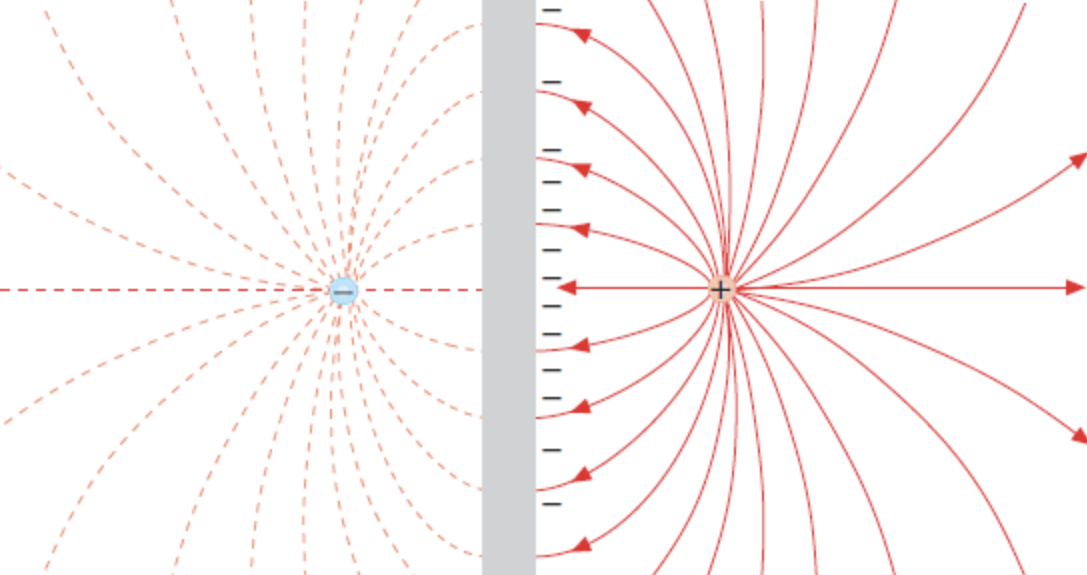
\includegraphics[width=0.4\linewidth]{figure/image19.png}
    \caption{Carica $q$ davanti a piano infinito}
    \label{fig:chapter_9_1}
\end{figure}

\subsection{Carica in presenza di una sfera conduttrice carica messa a terra}

Consideriamo una carica $q$ in posizione $\mathbf{r}$ rispetto all'origine $O$ del sistema, il quale è il centro di una sfera conduttrice messa a terra di raggio $a$. \\

Cerchiamo il potenziale $V(\mathbf{x})$ tale per cui $V(|\mathbf{x}| = a) = 0$. \\

\begin{figure} [h]
    \centering
    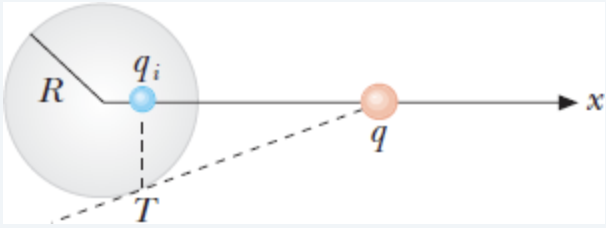
\includegraphics[width=0.4\linewidth]{figure/image20.png}
    \label{fig:chapter_9_2}
\end{figure}

Per simmetrica è evidente che l'immagine $q'$ sarà posizionata lungo il raggio che congiunge l'origine e la carica $q$. \\ Se la $q$ è \emph{esterna} alla sfera, la posizione $\mathbf{r'}$ della carica immagine sarà interna alla sfera ($\mathbf{|r'| < a}$). Il potenziale dovuto a $q$ e $q'$ risulta essere


\begin{equation*}
    V(\mathbf{x}) = \frac{q/4\pi \varepsilon_0}{|\mathbf{x} - \mathbf{r}|} + \frac{q'/4 \pi \varepsilon_0}{|\mathbf{x} - \mathbf{r'}|}
\end{equation*}

Dobbiamo scegliere $q'$ e $|\mathbf{r'}|$ in modo che il potenziale si annulli per $|\mathbf{x}| = a$. Scegliendo degli opportuni angoli e sfruttando alcune proprietà di similitudine tra triangoli si arriva facilmente al risultato. 

\begin{tcolorbox}[colback=yellow!10!white, colframe=orange!70!black, boxrule=0.8pt]
\begin{equation}
    q' = - \frac{a}{r}q \quad , \quad r' = \frac{a^2}{r}
\end{equation}
\end{tcolorbox}

La densità di carica indotta sulla superficie della sfera può essere calcolata dal tramite il gradiente del potenziale sulle superficie.

\begin{equation}
    \sigma = - \varepsilon_0 \nabla V(|\mathbf{x} = a|) = - \frac{q}{4 \pi a^2} \left ( \frac{a}{r} \right ) \frac{1 - \frac{a^2}{r^2}}{\left ( 1 + \frac{a^2}{r^2} - 2 \frac{a}{r} \cos \gamma \right )}
\end{equation} 

Dove $\gamma$ è l'angolo tra $\mathbf{x}$ e $\mathbf{r}$.\\

La carica totale indotta sul conduttore si trova facilmente utilizzando il teorema del Gauss. Immaginiamo una superficie gaussiana che avvolge in modo molto "aderente" il conduttore considerato, allora sappiamo che vale

\begin{equation*}
    \oint_{\Sigma} \mathbf{E} \cdot \mathbf{u}_n \ d\Sigma = \frac{Q_{\text{indotta}}}{\varepsilon_0}   
\end{equation*}

Ma dato che le cariche immagine devono essere interne al condensatore, si deve avere 

\begin{equation*}
    \oint_{\Sigma} \mathbf{E} \cdot \mathbf{u}_n \ d\Sigma = \frac{\sum q_{\text{immagine}}}{\varepsilon_0}   
\end{equation*}

Quindi 

\begin{tcolorbox}[colback=yellow!10!white, colframe=orange!70!black, boxrule=0.8pt]
\begin{equation}
    Q_{\text{indotta}} = \sum q_{\text{immagine}} 
\end{equation}
\end{tcolorbox}

Questo è un risultato del tutto generale. \\

La forza agisce sulla carica $q$ può essere calcolata in vari modi, il più semplice tra questi è trovare la forza tra la carica $q$ e la carica immagine $q'$.

\subsection{Carica in presenza di una sfera conduttrice carica isolata}

Consideriamo una sfera conduttrice carica con una carica $Q$ e una carica puntiforme q.\\

Da un punto di vista operativo possiamo pensare di avere inizialmente una sfera conduttrice messa a terra e una carica puntiforme $q$, in modo da utilizzare il metodo descritto sopra e trovare una carica immagine $q'$. \\

Possiamo poi scollegare da terra la sfera e aggiungere a questa una carica $(Q-q')$. Questo porta la sfera ad avere una carica totale $Q$. Per trovare il potenziale si nota che la carica aggiunta $(Q-q')$ si disporrà \emph{uniformemente} sulla superficie della sfera, poiché la forza elettrostatica dovuta a $q$ è bilanciata dalla carica $q'$. \\

\newpage

Allora il potenziale dovuto all'aggiunta della carica $(Q - q)$ sarà lo stesso di una carica puntiforme con la stessa carica situato nell'origine (questo per punti esterni alla sfera).

\begin{equation}
    V(\mathbf{x}) = \frac{1}{4 \pi \varepsilon_0} \left [ \frac{q}{|\mathbf{x} - \mathbf{r}|} - \frac{aq}{r|\mathbf{x} - \frac{a^2}{r^2} \mathbf{r}|} + \frac{Q + \frac{a}{r}q}{|\mathbf{x}|} \right ]
    \label{eq:7.4}
\end{equation}

Come nei casi precedenti per trovare la forza che agisce sulla carica $q$, basta trovare la forza tra $q$ e le due cariche immagine $q'$ e $(Q-q')$ .

\subsection{Carica in presenza di una sfera conduttrice a potenziale fissato}

Un altro problema che possiamo discutere semplicemente è quello una carica $q$ vicina a una sfera conduttrice a potenziale fissato $V$.\\

Possiamo agire esattamente come per il caso precedente, l'unica cosa è che al posto della carica $(Q-q')$ aggiungiamo la carica $4 \pi \varepsilon_0 Va$. Questo si vede dalla \ref{eq:7.4}, in quanto per $|\mathbf{x}| = a$ i primi due termini si cancellano (per costruzione) e l'ultimo termine deve essere uguale a $V$ come richiesto. 

\begin{equation}
    V(\mathbf{x}) = \frac{1}{4 \pi \varepsilon_0} \left [ \frac{q}{|\mathbf{x} - \mathbf{r}|} - \frac{aq}{r|\mathbf{x} - \frac{a^2}{r^2} \mathbf{r}|} \right ] + \frac{Va}{|\mathbf{x}|}
\end{equation}

\subsection{Sfera conduttrice in un campo elettrostatico uniforme}

Prima di considerare il caso vero e proprio, è necessario riportare alcune proprietà. \\

\begin{figure} [h]
    \centering
    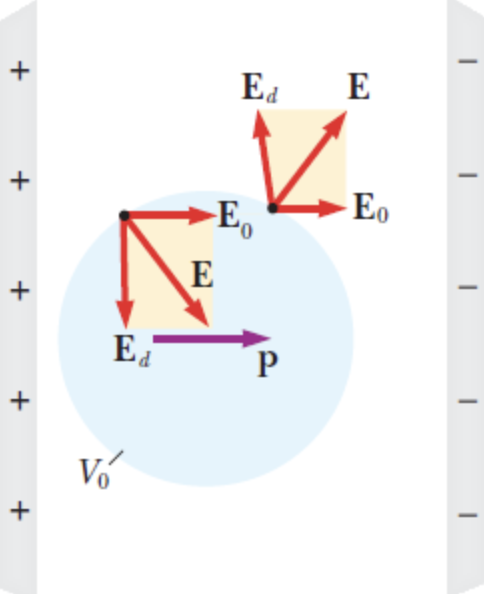
\includegraphics[width=0.25\linewidth]{figure/image21.png}
    \caption{Superficie equipotenziale del dipolo}
    \label{fig:chapter_9_3}
\end{figure}

\'E possibile dimostrare\footnote{Per la dimostrazione guardare \cite{ElettromagnetismoeOnde}, oppure farla a mano} che preso un campo elettrico uniforme $E_0$ e un dipolo parallelo al campo elettrico di momento di dipolo $\mathbf{p}$, esiste una superficie equipotenziale sferica con centro nel dipolo e raggio $R$, dove 

\begin{equation}
    R = \left ( \frac{p}{4 \pi \varepsilon_0 E_0} \right ) ^{1/3}
\end{equation}

Adesso possiamo passare al problema di nostro interesse.

Consideriamo una sfera conduttrice in un campo uniforme, la sua superficie deve essere equipotenziale; ma allora la situazione elettrostatica all'esterno della sfera si può calcolare supponendo di porre nel centro della sfera elettrostatica un \emph{dipolo immagine} con momento di dipolo $\mathbf{p}$ parallelo al campo e il cui momento è determinato dal raggio della sfera e dal valore del campo elettrostatico uniforme:

\begin{tcolorbox}[colback=yellow!10!white, colframe=orange!70!black, boxrule=0.8pt]
\begin{equation}
    p = 4 \pi \varepsilon_0 R^3 E_0
\end{equation}
\end{tcolorbox}

Il campo elettrostatico all'esterno della sfera è dato dalla sovrapposizione di $E_0$ e del campo del dipolo di momento $\mathbf{p}$. 

\begin{figure} [h]
    \centering
    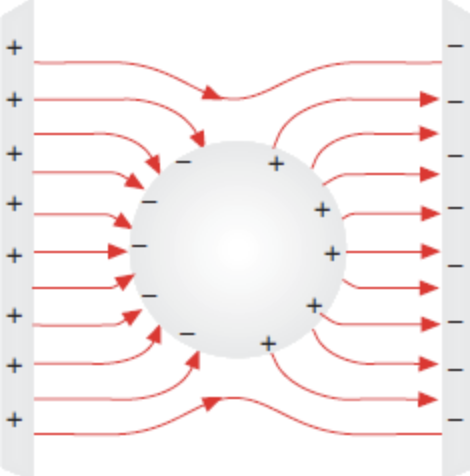
\includegraphics[width=0.35\linewidth]{figure/image22.png}
    \caption{Sfera conduttrice in un campo elettrico uniforme}
    \label{fig:chapter_9_4}
\end{figure}

In particolare il campo elettrico sulla superficie risulta essere 

\begin{equation}
    \mathbf{E} = - \nabla V = - \left ( \frac{\partial V}{\partial r} \right )_{r = R} \mathbf{u}_r = \left ( E_0 \cos \theta + \frac{2p \cos \theta }{4 \pi \varepsilon_0 R^3}\right) \mathbf{u}_r = 3 E_0 \cos \theta  \ \mathbf{u}_r 
\end{equation}

Inoltre possiamo trovare la densità di carica della sfera

\begin{equation}
    \sigma = E \varepsilon_0 = - \varepsilon_0 \frac{\partial V(|\mathbf{x}| = R)}{\partial r} = 3 \varepsilon_0 E_0 \cos \theta
\end{equation}

Si nota che l'integrale di superficie di questa quantità sparisce, quindi non c'è alcuna differenza tra una sfera messa a terra e una isolata. 

\subsection{Carica all'interno di una sfera conduttrice messa a terra}

Consideriamo una carica $q$ all'interno di una sfera conduttrice messa a terra di raggio $a$ a distanza $r$ dal centro della sfera.\\

La situazione è analoga al caso di una carica in presenza di una sfera conduttrice carica discusso sopra, l'unica differenza è che i ruoli della carica reale e della carica immagine sono invertiti, infatti si ha che per ricreare le condizioni al contorno possiamo considerare una carica immagine $q'$ a distanza $r'$ dal centro, dove

\begin{tcolorbox}[colback=yellow!10!white, colframe=orange!70!black, boxrule=0.8pt]
\begin{equation}
    q' = -\frac{r}{a} q \quad , \quad r' = \frac{a^2}{r}
\end{equation}
\end{tcolorbox}

\subsection{Energia del sistema con il metodo delle cariche immagine}

Quando si usa il metodo delle cariche immagine si deve fare attenzione, infatti potremmo farci prendere la mano e assumere che il sistema con il condensatore con condizioni al bordo e il sistema delle cariche immagine siano del \emph{tutto} identici, tuttavia questo \emph{non} è vero. \\

\emph{L'energia non è la stessa}. \\

Consideriamo l'esempio più semplice, quello di una carica $q$ in presenza di un piano conduttore messo a terra. \\
Se consideriamo il sistema ottenuto con il metodo delle cariche immagine, si ottiene che l'energia del sistema è 

\begin{equation*}
    U_{e_1} = - \frac{1}{4 \pi \varepsilon_0} \frac{q^2}{2d}
\end{equation*}

Se adesso, invece, consideriamo il sistema formato dalla carica e dal piano, otteniamo 

\begin{equation*}
    U_{e_2} = \frac{1}{2} \int V \ dq = - \frac{1}{4 \pi \varepsilon_0} \frac{q^2}{4d}
\end{equation*}

Si vede, allora, che $U_{e_1} \neq U_{e_2}$. \\

Riportiamo, allora, un metodo veloce e generale per trovare l'energia di un sistema con condizioni al contorno. \\

Sappiamo che per una distribuzione di cariche (nel caso continuo) vale 

\begin{equation*}
    U_e = \frac{1}{2} \int V \ dq
\end{equation*}

Nel nostro caso possiamo dividere le cariche che si trovano sul condensatore e le cariche reali esterne a quest'ultimo. 

\begin{equation*}
    U_e = \frac{1}{2} \int V_{\text{condensatore}} \ dq + \frac{1}{2} \int V_{\text{esterno}} \ dq
\end{equation*}

Tuttavia stiamo considerando un problema con condizioni al contorno, quindi $V_{\text{condensatore}} = V_0$ e la carica che si trova sul condensatore è esattamente $Q_{\text{condensatore}} = \sum q_{\text{immagine}}$. \\ Mentre il potenziale che si trova sulla p-esima carica reale risulta essere 

\begin{equation*}
    V_p = \sum _i \frac{1}{4\pi \varepsilon_0} \frac{q'_i}{r_{ip}} + \sum_j \frac{1}{4 \pi \varepsilon_0} \frac{q_j}{r_{jp}}
\end{equation*}

Dove $q'_i$ sono le cariche immagine e $q_j$ le cariche reali. 

Allora si ottiene che l'energia $U_e$ del sistema è  

\begin{tcolorbox}[colback=yellow!10!white, colframe=orange!70!black, boxrule=0.8pt]
\begin{equation}
    U_e = \frac{1}{2} V_0 \sum_i q'_i + \frac{1}{2} \sum_p q_p \left( \sum _i \frac{1}{4\pi \varepsilon_0} \frac{q'_i}{r_{ip}} + \sum_{j \neq p} \frac{1}{4 \pi \varepsilon_0} \frac{q_j}{r_{jp}}   \right)
\end{equation}
\end{tcolorbox}

\section{Metodo di separazione delle variabili}

In questa sezione andiamo ad "attaccare" direttamente l'equazione di Laplace, utilizzando il metodo di separazione delle variabili, uno dei metodi preferiti dei fisici per risolvere equazioni differenziali. \\

Il metodo è applicabile quando il potenziale o la densità di carica è specificata al contorno di una certa regione ed è chiesto di trovarne il potenziale all'interno.\\

La strategia di base è molto semplice: \emph{cerchiamo soluzioni esprimibili come prodotto di funzioni dove ciascuna di queste dipende solo da una coordinata}.\\

Tuttavia, i dettagli algebrici per trovare la soluzione particolare da quella generale, ponendo le condizioni al contorno, possono essere formidabili, per questo dedicheremo del tempo per capirne a fondo la matematica.

\subsection{Funzioni ortogonali e sviluppi}

Come accennato sopra, in questa sotto-sezione andremo a riportare alcuni mezzi matematici \emph{necessari} per capire a pieno i passaggi di alcune dimostrazioni e per \emph{risolvere un gran numero di problemi con condizioni al contorno}. \\

Iniziamo introducendo lo spazio $L^p$ \mkeyword{spazio $L^p$} come lo spazio delle funzioni a p-esima potenza sommabile. Si tratta di uno \emph{spazio funzionale} i cui elementi sono particolari classi di funzioni numerabili. \\ 

Gli $L^p$, con $1 \leq p \leq \infty$, sono spazi di Banach, e , in particolare, $L^2$ è uno spazio \mkeyword{funzioni a quadrato sommabile} di Hilbert\footnote{In realtà $L^2$ è \emph{l'unico spazio di Hilbert tra gli spazi $L^p$ }} ed è lo spazio delle funzioni a quadrato sommabile, cioè lo spazio delle funzioni tali per cui, in un intervallo $I = [a,b]$,  l'integrale del quadrato del loro modulo in $I$ è finito

\begin{equation*}
    \int_a ^b |f(x)|^2 dx < \infty
\end{equation*}

$L^2$ presenta un prodotto interno: 

\begin{tcolorbox}[colback=yellow!10!white, colframe=orange!70!black, boxrule=0.8pt]
\begin{equation}
    \langle f, g \rangle = \int_{X} f^* (x) g(x) dx
\end{equation}
\end{tcolorbox}

Dove $f,g \in L^2(X,\mathbb{C})$ e $f^* (x)$ è il complesso coniugato di $f(x)$ (ovviamente se $f$ è reale vale $f^*(x) = f(x)$). \\

Essendo $L^2$ uno spazio di Hilbert a avendone definito il prodotto interno, è sempre possibile andarne a trovare una base completa e ortogonale. Allora possiamo andare a considerare un generico intevallo $(a,b)$ e un insieme di funzioni reali o complesse $U_n(x)$, $n \in \mathbb{N}$, a quadrato sommabile ed ortogonali nell'intevallo $(a,b)$. \\

\newpage

La conduzione di ortogonalità delle funzioni $U_n (x)$ si traduce in 

\begin{equation}
    \int_a ^b U_n ^*(x)U_m(x) dx = 0 \qquad m \neq n
\end{equation}

Assumiamo che le funzioni siano normalizzate in modo che l'integrale sia l'unità. Allora le funzioni sono dette ortonormali, e soddisfano

\begin{equation}
    \int_a ^b U_n ^*(x)U_m(x) dx = \delta_{nm}
\end{equation}

Una funzione arbitraria $f(x)$, a quadrato sommabile nell'intervallo $(a,b)$, può essere sviluppata in una serie delle funzioni ortonormali $U_n(x)$. Se il numero di termini è finito,

\begin{equation*}
    f(x) \leftrightarrow \sum_{n = 1}^N a_n U_n(x)
\end{equation*}

allora possiamo domandarci quale sia la scelta "migliore" per i coefficienti $a_n$ per ottenere la rappresentazione "migliore" della funzione $f(x)$. Se "migliore" è definito in termini del minimo errore quadratico medio $M_N$:

\begin{equation*}
    M_N = \int_a ^b \left | f(x) - \sum_{n = 1}^N a_n U_n(x) \right |^2 dx
\end{equation*}

è facile dimostrare che i coefficienti sono dati da 

\begin{tcolorbox}[colback=yellow!10!white, colframe=orange!70!black, boxrule=0.8pt]
\begin{equation}
    a_n = \int_a ^b U_n^* (x) f(x) dx
    \label{eq:coefficienti_ortogonalità}
\end{equation}
\end{tcolorbox}

dove è stata utilizzata la \emph{condizioni di ortonormalità}. \\

Allora la rappresentazione in serie

\begin{equation*}
    \sum_{n=1} ^ \infty a_n U_n (x) = f(x)
\end{equation*}

con gli $a_n$ dati dalla \ref{eq:coefficienti_ortogonalità}, è detta \emph{convergere in media} a $f(x)$.\\

Adesso possiamo passare al vero e proprio metodo di separazione delle variabili.

\newpage

\subsection{Coordinate cartesiane}

Supponiamo di essere in coordinate cartesiane $(x,y,z)$, l'equazione di Laplace può essere scritta come

\begin{equation}
    \frac{\partial^2 V}{\partial x^2} + \frac{\partial^2 V}{\partial y^2} + \frac{\partial^2 V}{\partial z^2} = 0
    \label{eq:laplaciano_coordinate_polari}
\end{equation}

\emph{Assumiamo} che il potenziale possa essere rappresentato come il prodotto di tre funzioni dove ciascuna dipende solo da una coordinata:

\begin{equation}
    V(x,y,z) = X(x)Y(y)Z(z) 
    \label{eq:potenziale_prodotto}
\end{equation}

Sostituendo questa nella \ref{eq:laplaciano_coordinate_polari} e dividendo il risultato per \ref{eq:potenziale_prodotto} si ottiene 

\begin{equation}
    \frac{1}{X} \frac{d^2 X}{dx^2} + \frac{1}{Y} \frac{d^2 Y}{dy^2} + \frac{1}{Z} \frac{d^2 Z}{dz^2} = 0 
\end{equation}

Dato che si ha la somma di tre funzioni in tre variabili, affinché l'equazione sia valida si deve avere  

\begin{equation}
    \begin{cases}
    \frac{1}{X} \frac{d^2 X}{dx^2} = - \alpha ^2\\
    \\
    \frac{1}{Y} \frac{d^2 Y}{dy^2} = - \beta^2 \\
    \\
    \frac{1}{Z} \frac{d^2 Z}{dz^2} = \gamma ^2
    \end{cases}
\end{equation}

Dove

\begin{equation*}
    \alpha ^2 + \beta^2 = \gamma ^2
\end{equation*}

Le soluzioni delle tre equazioni differenziali sono $e^{\pm i \alpha x}, e^{\pm i \beta y}, e^{\pm\sqrt{\alpha^2 + \beta ^2} z}$, quindi per come abbiamo posto il potenziale:

\begin{tcolorbox}[colback=yellow!10!white, colframe=orange!70!black, boxrule=0.8pt]
\begin{equation}
    V(x,y,z) = e^{\pm i \alpha x} \ e^{\pm i \beta y} \ e^{\pm\sqrt{\alpha^2 + \beta ^2} z}
    \label{eq:soluzione_metodo_separazione_c}
\end{equation}
\end{tcolorbox}

A questo punto $\alpha$ e $\beta$ sono del tutto arbitrari. Di conseguenza la \ref{eq:soluzione_metodo_separazione_c} rappresenta, tramite sovrapposizione lineare, una classe molto ampia di soluzioni all'equazione di Laplace. \\ 

Per determinare $\alpha$ e $\beta$ è necessario imporre condizioni al contorno specifiche sul potenziale, cosa che porta, come accennato sopra, a conti non banali. \\

Si consiglia di guardare il \cite{ElettrodinamicaClassica}
per vedere alcuni esempi in cui si trovano le soluzioni particolari. 

\newpage

\subsection{Coordinate sferiche}

In coordinate sferiche $(r, \theta, \varphi)$ l'equazione di Laplace può essere scritta come 

\begin{equation}
    \frac{1}{r} \frac{\partial^2}{\partial r^2} (rV) + \frac{1}{r^2 \sin \theta} \frac{\partial}{\partial \theta} \left ( \sin \theta \ \frac{\partial V}{\partial \theta} \right ) + \frac{1}{r^2 \sin ^2 \theta} \frac{\partial^2 V}{\partial \varphi^2} = 0
\end{equation}

\emph{Assumiamo} che il potenziale possa essere rappresentato come il prodotto di tre funzioni dove ciascuna dipende solo da una coordinata:

\begin{equation}
    V(r, \theta, \varphi) = \frac{U(r)}{r} P(\theta) Q(\varphi)
\end{equation}

Sostituendo e dividendo per $r^2 \sin ^2 \theta /UPQ$, otteniamo 

\begin{equation}
    r^2 \sin ^2 \theta \left [ \frac{1}{U}\frac{d^2U}{dr^2} + \frac{1}{P r^2 \sin \theta} \frac{d}{d \theta} \left( \sin \theta \frac{dP}{d \theta}\right) \right] + \frac{1}{Q}\frac{d^2 Q}{d \varphi ^2} = 0
    \label{eq:7.19}
\end{equation}

La dipendenza da $\varphi$ è stata isolata all'ultimo termine. Di conseguenza, tale termine deve essere una costante, che chiamiamo $(- m^2)$:

\begin{equation}
    \frac{1}{Q} \frac{d^2 Q}{d \varphi^2} = - m^2
\end{equation}

Questa ha le soluzioni 

\begin{equation}
    Q = e^{\pm i m \varphi}
\end{equation}

Adesso facciamo delle considerazioni su $m$. La coordinata azimutale $\varphi$ ha periodo $2\pi$, quindi $V(r, \theta, \varphi) = V(r, \theta, \varphi + 2\pi)$, ma allora deve valere $Q(\varphi + 2 \pi) = Q(\varphi) $.\\ 
Quindi si ha 

\begin{equation*}
    Q(\varphi + 2 \pi) = e^{i m (\varphi + 2 \pi)} = Q(\varphi) e ^{i 2 \pi m} \implies e ^{i 2 \pi m} = 1 
\end{equation*}

Sappiamo che \emph{questo accade se e solo se $m \in \mathbb{Z}$} \\


Sostituendo questo risultato nella \ref{eq:7.19} e dividendo per $\sin^2 \theta$ si ottiene

\begin{equation}
    \frac{r^2}{U} \frac{d^2 U}{dr^2} + \frac{1}{P \sin \theta} \frac{d}{d \theta} \sin \theta \frac{dP}{d \theta} - \frac{m^2}{\sin ^2 \theta} = 0
    \label{eq:7.22}
\end{equation}

Adesso abbiamo isolato la dipendenza da $r$, quindi poniamo 

\begin{equation}
    \frac{r^2}{U} \frac{d^2 U}{dr^2} = l(l+1) \qquad l \in \mathbb{N} 
\end{equation}

La condizione $l \in \mathbb{N}$ adesso non è chiara, ma lo sarà tra poco. \\
La soluzione dell'equazione differenziale risulta essere

\begin{equation}
    U = A r^{l +1} + B r^{-l}
\end{equation}

Sostituendo nella \ref{eq:7.22}, otteniamo 

\begin{equation}
    \frac{1}{\sin \theta} \frac{d}{d \theta} \left ( \sin \theta \frac{d P}{d \theta} \right) + \left [ l(l+1) - \frac{m^2}{\sin ^2 \theta} \right ]P = 0
    \label{eq:7.25}
\end{equation}

\subsubsection{Equazione di Legendre e i polinomi di Legendre}

Come nei casi precedenti, nella \ref{eq:7.25} abbiamo isolato la dipendenza da $\theta$, tuttavia ora la soluzione non è banale. \\

L'equazione per $P(\theta)$ è di solito convenientemente espressa in termini $x = \cos \theta$, anziché di $\theta$ stesso. Ponendo $x = \cos \theta$, $-1 \leq x \leq 1$, $dx = - \sin \theta \ d \theta$, sostituendo otteniamo 

\begin{equation}
    \frac{d}{dx} \left [ (1 - x^2) \frac{dP}{dx} \right] + \left[ l (l+1) - \frac{m^2}{1-x^2} \right] P = 0
    \label{eq:Legrendre_gen}
\end{equation}

Questa equazione \mkeyword{equazione di Legendre generalizzata} prende il nome di equazione di Legendre generalizzata. \\

Prima \mkeyword{eqauzione ordinaria di Legendre} di considerare il caso generalizzato, però, descriviamo la soluzione dell'equazione differenziale ordinaria di Legendre con $m^2 = 0$, ciò nel caso ci sia \emph{simmetria azimutale}.

\begin{equation}
    \frac{d}{dx} \left [ (1 - x^2) \frac{dP}{dx} \right] +  l (l+1) P = 0
    \label{eq:7.27}
\end{equation}

\emph{Assumiamo che la regione di interesse comprenda tutto l'intervallo di $\cos \theta$, poli nord e sud inclusi}. \\

Assumiamo che la soluzione possa essere rappresentata con una serie di potenze nella forma:

\begin{equation}
    P(x) = \sum_{n= 0}^ {+ \infty} a_n x^n
\end{equation}


Si nota facilmente che valgono le seguenti relazioni:

\begin{align}
    \frac{d}{dx} x^2 \frac{dP(x)}{dx} = \sum_{n = 0} ^ {+ \infty} n (n + 1) a_n x^n \\
    \frac{d^2 P}{dx^2} = \sum_{n = 0}^{+ \infty} (n +2) (n+1) a_{n + 2}x^n
\end{align} 

Allora riscrivendo la \ref{eq:7.27} si ottiene

\begin{equation*}
    \sum_{n = 0} ^ {+ \infty} x^n [ (n+2)(n+1) a_{n+2} - n (n+1)a_n + l(l+1) a_n ] = 0
\end{equation*}

Affinché questa sia soddisfatta per qualsiasi $x$, ogni termine deve essere nullo. Allora 

\begin{equation}
    a_{n+2} = \frac{n(n+1) - l(l+1)}{(n+2)(n+1)} a_n
\end{equation}

Questa è una serie definita per ricorsione, tuttavia "salta" di due in due, quindi per descriverla in modo completo si devono definire sia $a_0$ sia $a_1$. \\

\newpage

\' E possibile dimostrare le seguenti proprietà della serie:

\begin{itemize}
    \item la serie converge per $x^2 < 1$, indipendentemente dal valore di $l$
    \item la serie diverge per $x = \pm 1$, \emph{a meno che termini}
\end{itemize}

Dato che stiamo considerando il caso $-1 \leq x \leq 1$, vogliamo che la serie termini. \\

Si nota che se poniamo 

\begin{equation*}
    l = n \qquad n\in \mathbb{Z}
\end{equation*}

Se $l$ è pari, allora esiste $p \in \mathbb{N}$ tale per cui $a_{2p} = 0$, se $l$ è dispari, allora esiste $k \in \mathbb{N}$ tale per cui $a_{2k +1} = 0$. Dato che nell'equazione compare $l(l+1)$ affinché la serie termini basta considerare $l \in \mathbb{N}$. Questo è il motivo per cui sopra abbiamo scelto $l \in \mathbb{N}$.\\

I polinomi per cui la serie termina prendono il nome \mkeyword{polinomi di Legendre} di polinomi di Legendre di ordine $l$, e sono indicati con $P_l (x)$. I primi polinomi di Legendre sono 

\begin{tcolorbox}[colback=yellow!10!white, colframe=orange!70!black, boxrule=0.8pt]
\begin{equation*}
    \begin{cases}
        P_0(x) = 1\\
        P_1(x) = x\\
        P_2(x) = \frac{1}{2}(3x^2 - 1)\\
        P_3(x) = \frac{1}{2}(5 x^3 - 3x)\\
        P_4(x) = \frac{1}{8} (35 x^4 - 30 x^2 + 3)
    \end{cases}
\end{equation*}
\end{tcolorbox}

\' E \mkeyword{formula di Rodrigues} possibile ottenere una rappresentazione compatta, nota come formula di Rodrigues , dei polinomi di Legendre:

\begin{tcolorbox}[colback=yellow!10!white, colframe=orange!70!black, boxrule=0.8pt]
\begin{equation}
    P_l (x) = \frac{1}{2^l l !} \frac{d^l}{dx^l} (x^2 - 1)^l
    \label{eq:Rodrigues}
\end{equation}
\end{tcolorbox}

Allora \emph{se siamo nel caso di simmetria azimutale}, la soluzione generale del potenziale risulta essere 

\begin{tcolorbox}[colback=yellow!10!white, colframe=orange!70!black, boxrule=0.8pt]
\begin{equation}
    V(r, \theta) = \sum_{l = 0} ^ {+ \infty} \left ( A_l r^l + B_l \frac{1}{r^{l+1}} \right) P_l (\cos \theta)
\end{equation}
\end{tcolorbox}

A questo punto $A_l$ e $B_l$ sono del tutto arbitrari e per determinarne il valore è necessario imporre condizioni al contorno specifiche sul potenziale. \\

\emph{Per far questo ci viene in aiuto un' importante proprietà dei polinomi di Legendre}, infatti è possibile dimostrare che \emph{i polinomi di Legendre costituiscono un sistema ortogonale completo in $L^2(I,\mathbb{R})$, con $I = [-1,1]$, rispetto al prodotto interno} e in particolare vale che 

\begin{equation}
    \int_{-1}^1 P_{l'} (x) P_{l}(x) \ dx = \frac{2}{2l +1} \delta_{l'l}
\end{equation}

Questo semplifica di molto il processo che permette di trovare i valori di $A_l$ e $B_l$, soprattutto quando il potenziale è specificato su una o più superfici sferiche. \\

Supponiamo, infatti, di avere un sistema dove è conveniente usare le coordinante sferiche ed è presente una simmetria azimutale. \\
Supponiamo che venga chiesto di risolvere il problema del potenziale all'esterno (o all'interno) di una superficie sferica in cui è specificato il potenziale al bordo $V_0 ( \theta)$. \\

Dato che stiamo considerando il potenziale all'esterno (o all'interno) i termini $A_l$ si annullano in quanto abbiamo posto che il potenziale all'infinito tende a zero e se esistesse $l$ tale per cui $A_l \neq 0$, allora il potenziale "esploderebbe" per $r \to \infty$ (nel caso interno, si annullano i termini $B_l$ in quanto si considera anche l'origine).\\

Allora vale 

\begin{equation*}
    V(r, \theta) = \sum_{l = 0} ^ {+ \infty} \left ( B_l \frac{1}{r^{l+1}} \right) P_l (\cos \theta)
\end{equation*}

Moltiplicando a sinistra e a destra per $P_{l'} (\cos \theta) \sin \theta$ e integrando in $\theta$ tra $0$ e $\pi$ si ottiene 

\begin{equation*}
\begin{aligned}
    \int_0^{\pi} V(r,\theta)\, P_{l'}(\cos\theta)\, \sin\theta \, d\theta
    &= \int_0^{\pi} \sum_{l=0}^{+\infty} \left( B_l \frac{1}{r^{l+1}} \right)
       P_l(\cos\theta) P_{l'}(\cos\theta) \sin\theta \, d\theta \\
    &= \sum_{l=0}^{+\infty} \left( B_l \frac{1}{r^{l+1}} \right)
       \int_0^{\pi} P_l(\cos\theta) P_{l'}(\cos\theta) \sin\theta \, d\theta
\end{aligned}
\end{equation*}

In particolare questa relazione è valida anche sul contorno, dove è specificato il potenziale

\begin{equation*}
    \int_0 ^{\pi} V_0(\theta) P_{l'} (\cos \theta) \sin \theta \ d \theta = \sum_{l = 0} ^ {+ \infty} \left ( B_l \frac{1}{R^{l+1}} \right) \int_0 ^{\pi} P_l (\cos \theta) P_{l'} (\cos \theta) \sin \theta \ d \theta
\end{equation*}

Facendo il cambio di variabile $x = \cos \theta$ otteniamo 

\begin{equation*}
    \int_{-1} ^{1} V'_0(x) P_{l'} (x) \ d x = \sum_{l = 0} ^ {+ \infty} \left ( B_l \frac{1}{R^{l+1}} \right) \int_{-1} ^{1} P_l (x) P_{l'} (x) \ d x = \frac{2}{2l +1} \frac{1}{R^{l'+1}} B_{l'}
\end{equation*}

Questo perché ci siamo ricondotti al prodotto interno e abbiamo sfruttato l'ortogonalità dei polinomi di Legendre. Si ottiene così la relazione 

\begin{tcolorbox}[colback=yellow!10!white, colframe=orange!70!black, boxrule=0.8pt]
\begin{equation*}
    B_l = \frac{2l +1}{2} R^{l+1} \int_{-1} ^{1} V'_0(x) P_{l} (x) \ d x
\end{equation*}
\end{tcolorbox}

\newpage

Quindi per trovare i termini basta andare a risolvere gli integrali. Spesso, però, è sufficiente risolvere solo alcuni integrali, infatti si nota che compare il prodotto tra $P_l(x)$ e $V_0 ' (x)$ e se quest' ultimo è una funzione a quadrato sommabile (come un polinomio), allora è esprimibile come combinazione lineare di \emph{alcuni} polinomi di Legrendre, allora basterà calcolare gli integrali solo per gli $l$ che compaiono nella combinazione. \\

Si riporta anche l'espressione (ottenuta in un modo del tutto analogo)
per trovare i coefficienti nel caso interno alla superficie.

\begin{tcolorbox}[colback=yellow!10!white, colframe=orange!70!black, boxrule=0.8pt]
\begin{equation}
    A_l = \frac{2l +1}{2 R^l}  \int_{-1} ^{1} V'_0(x) P_{l} (x) \ d x
\end{equation}
\end{tcolorbox}
